\documentclass[10pt,a4paper]{article}
\usepackage{geometry}
\usepackage[IL2]{fontenc} 
\usepackage[utf8]{inputenc}
\usepackage{graphicx}
\usepackage{url} 
\usepackage{hyperref} 
\usepackage{cite}


\pagestyle{headings}

\title{Machine Learning in Search Engines: Improving Information Selection for Users\thanks{Semestrálny projekt v predmete Metódy inžinierskej práce, ak. rok 2023/24, vedenie: Ing. Mohammad Yusuf Momand, MSc.}}

\author{Marián Kurčina\\[2pt]
	{\small Slovenská technická univerzita v Bratislave}\\
	{\small Fakulta informatiky a informačných technológií}\\
	{\small \texttt{xkurcinam@stuba.sk}}
	}

\date{\small 30. október 2023} 



\begin{document}

\maketitle

\begin{abstract}
In an era of the internet, search engines have become the gateway to knowledge. They play a prime role in connecting users with the information they seek, but achieving optimal information selection remains a difficult challenge. From personalized search results that align with individual preferences to context-sensitive responses that adapt to specific needs, machine learning is driving improvements in relevance and user satisfaction. This article delves into the impact of machine learning in search engines and how it is changing the way information is selected and presented to users. We will explore the evolution of search engines, the integration of neural networks, and the incorporation of user behaviour data in shaping search outcomes.
\end{abstract}



\section{Introduction}
In today's digital age, the internet has revolutionized how we access information. With the projected surge of data worldwide from 33 zettabytes in 2018 to 175 zettabytes by 2025\cite{DJR-Digitalization}, it can be a daunting task for the average online user to go through and locate the desired information. From the beginning stages of the internet, search engines have been essential in providing users with the ability to search and filter the information available online. However, with the exponential growth in the amount of data available, search engines have had to adapt to meet the ever-changing demands of users by providing the most relevant and accurate results. The solution to this problem was found through the implementation of machine learning. The integration of machine learning in search engines has revolutionized the search process, providing users with personalized results based on their preferences.  In this article, we will discuss how machine learning shaped search engines, but first, we have to look into what search engines are and how they work. 

\section{Search Engines}
Search engines\cite{SEReleC} are tools that enable users to locate information on the internet. These search engines provide results that can consist of various types of content, such as web pages, images, videos, files, and other types of information. The thousands of web pages are processed and presented in the form of a list called "Search results". The search results can contain thousands of pages with the most suitable being at the top. Working of a search engine consists of 3 main processes:
\begin{itemize}
\item web crawling
\item indexing
\item searching
\end{itemize}

Web crawling \cite{WebCrawler} is a process in which a web crawler, program/software or programmed script, systematically browses the Internet. The Internet has a graphical structure, which means the page may be connected to other pages through URL links. A web crawler utilizes a graphical structure to navigate the vast expanse of the Internet. During its journey, it may discover and visit new web pages, which are subsequently added to a local repository. While traversing the World Wide Web, a web crawler systematically retrieves information about various web pages and subsequently archives it in its designated database (indexing). Indexing is the most important part of the whole process with size of the indexes of the biggest search engines in billions.\ref{Table 1} The last part of the searching process is searching itself. The browser uses a search interface, which connects the user and the database, it helps with searching through the database and provides the user with a search result page. 

\begin{figure}[h]
\center
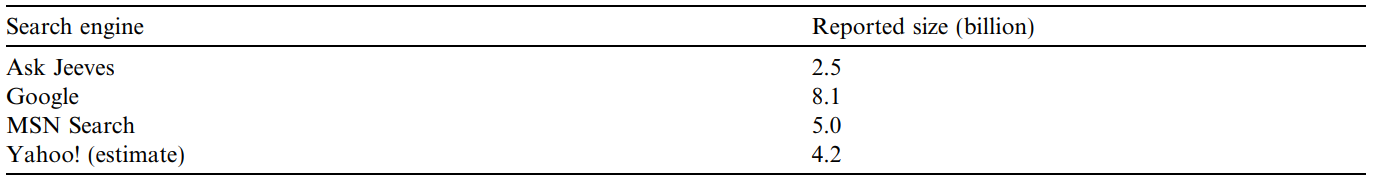
\includegraphics[scale=0.5]{table1.png}
\caption{Reported size of each Web search engine index\cite{SPINK20061379}}
\label{Table 1}
\end{figure}

\subsection{Types of search engines}
There are 4 types of search engines.\cite{TK-SE}They are:
\begin{itemize}
\item \textbf{Crawler based search engines} 

The listings are generated automatically by crawling through the internet. Changes made to web pages can affect the listings and the rank they will be presented at in search results. The examples of crawler based search engines are Google and Bing. 

\item \textbf{Human powered directories}

Listings depend on human submissions made by the page owner. The submissions contain an address, title and a description of their site. These submissions are then approved or denied by editors. The advantage of this type of search engine is a better quality of web pages, but on the downside, after committing any changes to the page it has to go through a process of submitting again. 

\item \textbf{Hybrid search engines}

Hybrid search engines use features from crawler-based search engines as well as from human-powered directories. This makes the search process more effective.

\item \textbf{Meta search engines}

Metasearch engines use search results from other search engines. The results are combined and listed according to their relevance across all used search results. MetaCrawler is one example of a Meta search engines.
\end{itemize}

\section{History of search engines}
\paragraph{Historical connections.}
The first tool\cite{History} for searching through content online, named Archie, was created in 1990 by Alan Emtage, Bill Heelan and J. Peter Deutsch. Archie did not index the contents of the sites, with the amount of data that wasn't needed, it was possible to search manually. Then in 1993, Matthew Gray produced the first web robot, World Wide Web Wanderer, which he used to generate an index called "Wandex". His purpose was to measure the size of the World Wide Web. The same year the Aliweb search engine was created. This search engine as Archie wasn't using a web robot, instead, it depended on notifications from website administrators. 
In late 1993 the Jump Station was created, a search engine which used a web robot to find web pages and to build its index. The next advancement came in the year 1994 when the WebCrawler was created. Unlike its predecessors it allowed its users to search for any word on a webpage. It was also the first one to be widely known by the public. During the early 2000s, Google emerged as the leading player in the market. The company achieved better search results with an innovation called PageRank \cite{rogers2002google}.

\section{Machine Learning}
The solution to better and more relevant information selection is machine learning. Machine learning is a branch of computer science that makes computers learn without being directly programmed. It learns by improving its performance by working with training data and adapting according to its results. (As shown in the Figure \ref{Diagram 1}) After learning it is supposed to be able to work with any set of data provided to it. There are 3 main types of learning\cite{QGKL-ML}: 


\begin{itemize}
\item \textbf{Supervised learning} 

With this type of learning the value of outcome is known for each observation. 

\item \textbf{Unsupervised learning} 

Opposite to supervised learning, the outcome values are not known. An algorithm has to identify common characteristics within data without any reference.

\item \textbf{Reinforcement learning} 

The system learns through trial and error over time and gets either positive or negative feedback according to their performance. through time it self adapts and gets better at a task.
\end{itemize}

The learning of a system itself is done through learning algorithms. The most famous algorithm used for machine learning is an artificial neural network which will be briefly introduced to you below. 

\begin{figure}[h]
\center
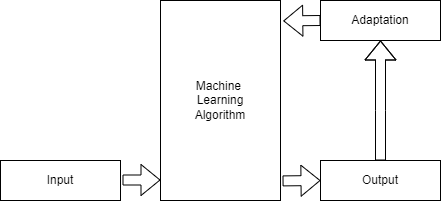
\includegraphics[scale=0.5]{diagram1.png}
\caption{Machine learning process}
\label{Diagram 1}
\end{figure}

\subsection{Neural Networks} 
Artificial neural networks \cite{zou2009overview} are inspired by the functioning of the brain and its neurons (therefore its name).  The network is made of 3 types of neuron layers: input layer, hidden layer and output layer. Neurons are connected and based on a connection strength they give output to another layer of neurons. The learning process consists of letting the system change connection strength between neurons according to the output. Learning can be supervised, unsupervised or also reinforced.(An example of such a network can be seen at figure\ref{Diagram 2})

\begin{figure}[h]
\center
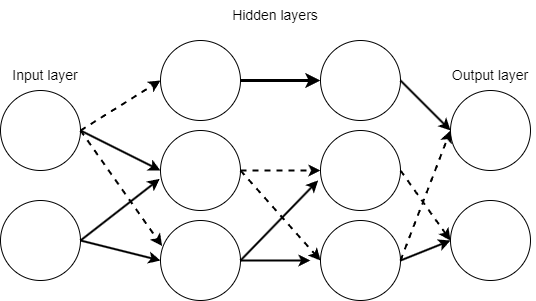
\includegraphics[scale=0.45]{diagram2.png}
\caption{Artificial neural network}
\label{Diagram 2}
(dashed lines represent weaker connection)
\end{figure}

\section{Applications of Machine Learning in Search Engines}
Machine Learning can be applied in multiple ways to improve searching experience\cite{Sunny:MLiSE}:

\begin{itemize}
\item \textbf{Better search ranking results} 
\item \textbf{Query understanding}
\item \textbf{Weider search selection} 
\item \textbf{More relevant ads} 
\item \textbf{Pattern recognition} 
\item \textbf{Detecting unwanted messages}
\item \textbf{Search related features} 
\item \textbf{Better crawlers} 
\item \textbf{More effective work} 
\end{itemize}

\subsection{Better search ranking results}
\cite{Sunny:MLiSE}Machine learning can substantially improve search results, by making them more personalized, by detecting duplicates and stolen content. Without machine learning, the law would have to be reinforced manually, which would be practically impossible. Identifying stolen content is this way automatic. Personalization plays a dramatic role in better search results. Providing a user with personalized content searching for desired content takes less time and makes searching more pleasant.
\subsection{Query understanding}
\cite{Sunny:MLiSE}While searching and writing expressions in a search engine, the search engine needs to understand what is the user trying to ask. If it can't understand the question the search results won't be helpful. This is where machine learning helps. Machine learning can identify and correct spelling mistakes and it can identify and work with synonyms. 
\subsection{Weider search selection}
\cite{Sunny:MLiSE}Thanks to machine learning, text searching isn't the only search option. Machine learning can understand multiple other inputs, like photo search, music search or voice search. Through long learning, search engines now provide more ways to search. By taking a photo, the search engine finds similar photos and identifies an object. It makes searching also accessible to people who find it difficult to write, by having a build in feature that converts a speech to text. Machine learning takes a part in that too. 
\subsection{More relevant ads}
\cite{Sunny:MLiSE}The companies owning search engines get revenue from advertisements that they display on their websites. By showing more relevant ads to the users the chance of them clicking on them is higher which is beneficial for the search engines, but also for the company providing the product or service, with their sales being greater.  Machine learning can identify the correct group to target and then show them the advertisement. 
\subsection{Pattern recognition}
\cite{Sunny:MLiSE}Search engines use machine learning to detect patterns, which can help in a multitude of ways. Search engines can recognize spam and unwanted messages, but also they're able to recognize handwritten text and other patterns which help with analysing the content on the web pages and thus can eliminate low-quality pages from its ranking page. 
\subsection{Detecting unwanted messages}
\cite{Sunny:MLiSE}As discussed in the last paragraph, machine learning can detect unwanted content and eliminate it before it gets to the user. One of the biggest problems with children having access to the internet is the explicit content they might be exposed to. The search engines allow parents to turn on a kids mode which filters content and removes anything not suitable for young.
\subsection{Search related features}
\cite{Sunny:MLiSE}Machine learning is used to enhance the search experience, with search features like related searches, recommended content or user classification. With machine learning content is recommended to users according to the stuff they would enjoy. User classification helps with that. The search engine gets to know what kind of user you are, which is then used to recommend more precise content for them. 
\subsection{More effective work}
\paragraph{People and work.}I see a possibility of machine learning helping with work and planning. Machine learning could help with planning a sprint or even replacing a scrum master. It is capable of doing small tasks and it can help with information search which would make work more easy and more effective. All the said features can help with workflow. 


\section{Compications with implementation}
\paragraph{Sustainability and ethics.}
\cite{FootprintofAI}As with everything, the implementation of machine learning and AI in search engines has some complications. The learning process and the actual running of the programs are costly. If Google was to change their whole system to AI it would cost them tens of billions of dollars. Afterwards, the cost of electricity required for its running would be another problem. The estimated power consumption would be around 29.2 terawatt-hours per year. This consumption level is equivalent to the consumption of Ireland and would be double the company's total energy consumption of 15.4 terawatt hours in 2020 \cite{Google2021}. With the world trying to be more eco-friendly, this change could generate a lot of public rage.

\section{Conclusion} 
In conclusion, I think the addition of Machine learning in search engines has many advantages even though the troubles of its implementation. Since its implementation, there have been many ways it has helped with searching and it is a perfect solution to increase of data available on the World Wide Web.  

\bibliography{literatura}
\bibliographystyle{plain} 
\end{document}
